%!TEX program=luatex

\newpage
\section{Présentation de l'application "Feedny"}
Après avoir compléter les différents modules qui composent notre système, nous avons procéder à l'intégration de ces derniers dans une application mobile multi plate-formes (Androïd et IOS) dans l'optique de permettre à l'utilisateur de bénéficier de chaque fonctionnalité.

L'expérience utilisateur au sein de notre application est étudier pour optimiser la navigation entre les différents espaces. L'application est très intuitifs et conçu afin d'attirer les utilisateurs le plus de temps possible.

La phase d'implémentation a été divisée en deux phases, le développement Back-end de l'API qui est la pièce motrice de l'application et qui intègre tout les modèles de classification, résumé et recommandation, et le développement de l'interface utilisateur sous forme d'une application mobile.

\begin{figure}[H]
    \centering
    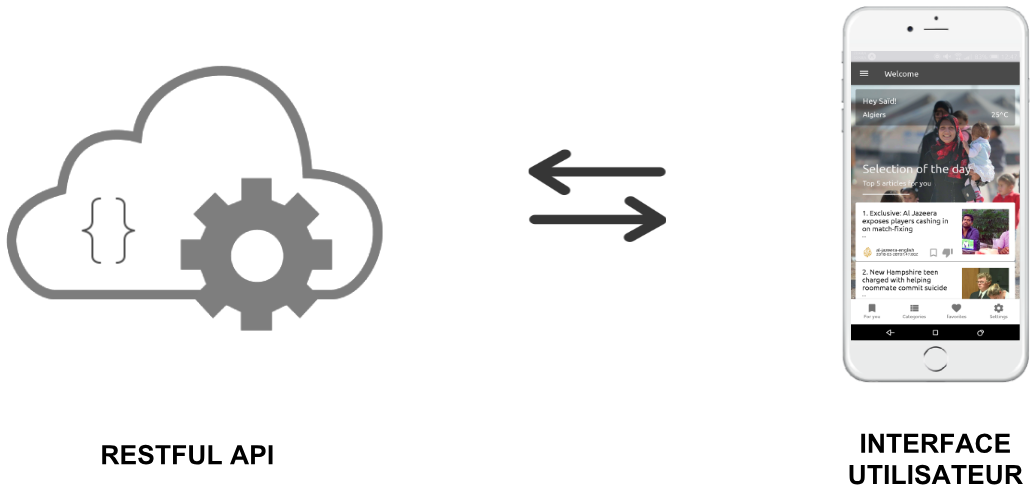
\includegraphics[height=132pt,width=270pt]{img/chapter4/frontbackend.png}
    \caption{Logos des langages de programmations utilisés}
    \label{}
\end{figure}

Nous allons présenter chaque étape d'implémentation dans ce qui suit.

    \subsection{Back-end}
    La partie "métier" de l'application consiste en une REST API qui intègre tout les modules. L'API reçoit les requêtes des utilisateurs à travers l'interface, et retourne une réponse via le protocole HTTP.

    Elle est composée de TROIS principaux modules :
        \begin{itemize}
            \item Extraction d'articles
            \item Géstion de la base de données
            \item GESTION DE
        \end{itemize} 
    Nous allons expliquer en détails le fonctionnement de chaque module dans la partie suivante.

        \subsubsection{Extraction d'articles}
        Le composant clés de notre système est l'article de presse, ce dernier se trouve un peu partout sur les revues de preese en ligne. À cet effet, nous avons implémenter une fonctionnalité qui permet d'extraire des articles de presse de différentes sources dans les deux langues.

        L'extraction d'articles de presse peut être personnalisée selon le besoin, on peut choisir à partir des catégories, région, pays, etc.

        Lors de l'extraction d'un article, nous allons récupéré toutes les informations relative à ce dernier tels que : le contenu de l'article, le titre, l'auteur, l'horaire de publication, etc.

        Le module d'extraction d'article de presse peut être invoquer juste en saissant une requete dans le navigateur ou en visitant la page principale de notre application, et on aura la réponse sous le format JSON, comme dans l'exemple suivant qui monte une extraction par nom de source :

\begin{lstlisting}[style=api] 
  http://feedny.io/api/articles/add/sources=al-jazeera-english
\end{lstlisting}
        
        ou encore par catégorie :
\begin{lstlisting}[style=api] 
  http://feedny.io/api/articles/add/categories=sport,health
\end{lstlisting}  

        \subsubsection{Géstion de la base de données}
        Le module de géstion de la base de données s'occupe de l'insertion, la suppression, la recherche et la mise à jour des articles et des profils utilisateurs.

        Chaque appel de l'API implique systématiquement une opération implicite sur la base de données. Elle est composée, comme cité dans \autoref{}, de deux collection : Articles et Profils. 

        \begin{enumerate}[leftmargin=*]
            \item\textbf{Gestion de la collection d'Articles}\\
            Après extraction d'un article de presse, il sera stocké dans un document qui apparient à la collection Articles dans notre base de données NoSQL (la structure d'un document Article a été présentée dans \autoref{}) afin de faciliter la recherche et de remédier à la lenteur du débit internet. 

            La recherche peut se faire avec n'importe quel attribut d'un article, et c'est l'un des plus grand avantages des base de données NoSQL. Les articles peuvent aussi avoir une structure différentes, et on peut stocké, également, des images et du son, s'il y-en a.

            On peut également proposer des articles à un utilisateur, en utilisant son vecteur de probabilité de sélection et ses sources préférées : 
\begin{lstlisting}[style=api] 
  http://feedny.io/api/profiles/onload/username=yankheloufi
\end{lstlisting} 
            
            \item\textbf{Gestion de la collection de Profils}\\
            La stucture des profils utilisateurs est très dynamique, elle est différentes d'un utilisateur à un autre. Les utilisateurs peuvent avoir plusieurs préférences et source favorites comme ils peuvent ne pas avoir. La gestion des profils est également effectué à partir de l'API, un nouvel utilisateur est ajouter de la façon suivante :   
\begin{lstlisting}[style=api] 
  http://feedny.io/api/profiles/add/profile=username::password::user@hey.com::sport,religion::bbc-news,echourouk
\end{lstlisting} 
            
            Et le profil peut être également mis à jour de la manière qui suit : 
\begin{lstlisting}[style=api] 
  http://feedny.io/api/profiles/update/profile=username::preferences+algeria
\end{lstlisting}            
        \end{enumerate} 

    \subsection{Front-end}
    Dans le monde du developpement web et mobile, nous recherchons toujours des cycles de développement très courts, des délais de déploiement réduits avec une meilleure performance.

    Une technologie très récente (2016) se trouve au beau milieu de ces exigences, le developpement d'application mobile hybride, en utilisant des techniques et des languages de programmations très répandus parmi les développeurs web (comme JavaScript ou HTML5 et CSS) enveloppées dans un Framework lui permettant de fonctionner nativement sur n'importe quel appareil et système d'exploitation (Andoir et IOS).

    Ils existent plusieurs Frameworks d'applications mobiles hybrides, mais React-native \autoref{} developpé par \emph{Facebook}, et jusqu'à l'écriture de ces lignes, reste le plus performant et le plus evolutifs tout en restant stable. On peut cité quelques points forts de React-native : 
        \begin{itemize}
            \item Open source, communauté ne cessent de s'agrandir,
            \item Facebook continue à investir dans sa croissance,
            \item Les composants réutilisables,
            \item Compatibilité avec les APIs, les SGBDs et les extensions tiers,
            \item Moins d'utilisation de la mémoire,
            \item ...
        \end{itemize}
    Tout ces arguments nous ont poussé à choisir React-native comme Framework pour developper notre application mobile. 

    \subsubsection{Fonctionnalités disponibles}
    Deux méthode d'utilisation de notre application sont disponible: Avec authentification, Sans authentification. La personnalisation des recommandations en dépendra.
    \begin{enumerate}[leftmargin=*]
        \item\textbf{Avec authentification (personnalisé)}\\
        Si l'utilisateur s'authentifie, la version personnalisée de notre application lui sera accessible et pourra dès la première connexion choisir ses catégories et ses sources favorites afin de construire son profil utilisateur.

        À partir de là, les articles proposés sont choisis en fonction de ses préférences, et les recommandations seront de plus en plus raffinées avec l'utilisation de l'application.

        Les utilisateurs de "Feedny" auront comme fonctionnalités:  
        \begin{itemize}
            \item \textbf{Catégorisation automatique d'articles :}\\
            Les articles sont classifiés dans différentes catégories suivant le sujet traité.
            \item \textbf{Résumé automatique :}\\
            Au lieu de lire un article complet, l'utilisateur aura un résumé généré automatiquement à partir de l'article qui lui permettra de retrouver tout les faits importants décrit dans l'article.
            \item \textbf{Traduction automatique :}\\
            l'utilisateur aura la possibilité d'avoir une traduction de l'article en cours de lecture.
            \item \textbf{Favoriser un article, une revue ou une catégorie :}\\
            L'utilisateur pourra aussi marquer un article, une source ou une catégorie précise d'articles comme favorite.
            \item \textbf{Mentionner la satisfaction :}\\
            Il aura la possibilité d'ajouter une mention de préférence "J'aime" ou "Je n'aime pas" sur la recommandation.
            \item \textbf{Recherche d'articles :}\\
            l'utilisateur aura la possibilité de faire une recherche spécifique des articles, et ceux en se basant soit sur : une recherche basé mots clés, une recherche basé sur une catégorie ou une recherche selon la source de l'article. 
            \item \textbf{Consultations des articles recommandés :}\\
            L'interface offrira la possibilité de consulter tout les détails concernant l'article (auteur, date de publication, etc.) 
        \end{itemize}
        Dès la connexion de l'utilisateur, ce dernier peut s'identifier en utilisant un nom d'utilisateur et un mot de passe ; sinon il utilisera les services non personnalisés du système qui sont présentés dans le point suivant.\\

        \item\textbf{Sans authentification (non personnalisé}\\
        Dans le cas où l'utilisateur ne souhaite s'identifier, la version non personnalisé sera entièrement accessible et il pourra :
        \begin{itemize}
            \item \textbf{Recommandation basée similarité :}\\
            Dans le cas non personnalisé, la recommandation se basera uniquement sur l'article consulté et lu et les différents articles disponible dans la base de données.    
            \item \textbf{Consultation des articles suggérés :}\\
            l'utilisateur pourra en effet au moment même ou il lit un article, d'avoir une suggestion d'autres articles jugés similaires par le système.
            \item Toutes les autres fonctionnalités de la version Personnalisé qui n'utilisent pas le profile utilisateur sont également disponible.
        \end{itemize}
    \end{enumerate}
    \vspace*{0.7cm}
    Nous allons voir maintenant, les différentes interfaces de noter application.
    \subsubsection{Authentification}
    L'utilisateur peut créer un compte afin de s'authentifier, il peut s'inscrire en utilisant son compte \emph{Google}, \emph{Facebook} ou \emph{Twitter}. 
        \begin{figure}[H]
            \centering
            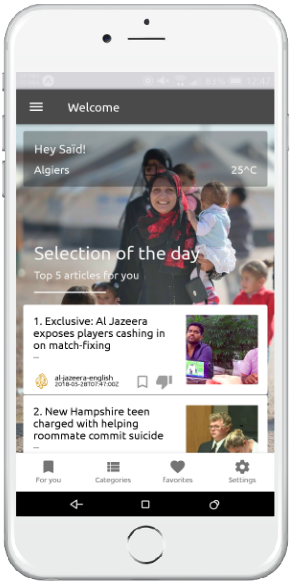
\includegraphics[height=200pt,width=100pt]{img/chapter4/feedny/feedny.png}
            \caption{Espace d'authentification de "Feedy"}
            \label{}
        \end{figure}

    % \subsubsection{Interface principale}
    % L'espace principale de "Feedny" contient plusieurs 
    % \subsubsection{Favoris}
    % \subsubsection{Catégories}
    % \subsubsection{Article}

 
